\documentclass{article}
\usepackage[utf8]{inputenc}
\usepackage{amsmath}
\usepackage{amssymb}
\usepackage{graphicx}
\usepackage{framed}
\renewcommand{\familydefault}{\sfdefault}
\usepackage{listings}
\usepackage{color}

\definecolor{dkgreen}{rgb}{0,0.6,0}
\definecolor{gray}{rgb}{0.5,0.5,0.5}
\definecolor{mauve}{rgb}{0.58,0,0.82}

\lstset{frame=tb,
  language=Python,
  aboveskip=3mm,
  belowskip=3mm,
  showstringspaces=false,
  columns=flexible,
  basicstyle={\small\ttfamily},
  numbers=none,
  numberstyle=\tiny\color{gray},
  keywordstyle=\color{blue},
  commentstyle=\color{dkgreen},
  stringstyle=\color{mauve},
  breaklines=true,
  breakatwhitespace=true,
  tabsize=3
}

\title{Assignment 1}
\author{Tanuj Kumar kumarta3 1002197133}
\date{September 2017}

\begin{document}

\maketitle

\section{Question 1}

\subsection{1 a}
Let $\delta(t)$ be the one dimensional impulse function at $t$. Define a 2D space with axes $x$ and $y$. 
\\\\
\noindent
Then, we can define the \textbf{two-dimensional impulse function} as:

$$\delta(u,v) = 
\begin{cases}
1 & (u,v) = (0,0) \\
0 & \text{else}
\end{cases}$$

\noindent
Where $u$ and $v$ are spatial two-dimensional coordinates on the $x$ and $y$ axes respectively. If we were to define two separate 1D impulse functions $\delta_{x}(u)$ and $\delta_{y}(v)$, we could also write our 2D impulse function as a product of these:

$$\delta(u,v) = \delta_{x}(u)\delta_{y}(v)$$

\subsection{1 b}

Consider a 2D impulse located at coordinates $u = m$ and $v = n$. Our 2D impulse function at position $(m,n)$ is simply:

$$\delta_{(m,n)}(u,v) = \delta(u - m, v - n)$$

\noindent
We can show this is the case: $\delta_{(m,n)}(m,n) = \delta(m-m,n-n) = \delta(0,0) = 1$, as required.

\subsection{1 c}

Python code:

\begin{lstlisting}
import matplotlib.pyplot as plt
from mpl_toolkits.mplot3d.axes3d import Axes3D, get_test_data
from matplotlib import cm
import numpy as np

def pulse(m, n, tups):
	img = np.zeros(shape=(m,n))
	for t in tups:
		img[t[0]-1][t[1]-1] = 1
	return img

pops = [(10,20),(20,40),(30,60),(40,80),(50,100),(60,80),(70,60),(80,40),(90,20)]
impulseimg = pulse(100, 200, pops)

fig = plt.figure(figsize=plt.figaspect(0.5))

ax = fig.add_subplot(1, 2, 1, projection='3d')

X = np.arange(1,201,1)
Y = np.arange(1,101,1)

X, Y = np.meshgrid(X, Y)

surf = ax.plot_surface(X, Y, impulseimg, rstride=1, cstride=1, cmap=cm.coolwarm, linewidth=0, antialiased=False)

ax.set_zlim(-0.01, 1.01)
fig.colorbar(surf, shrink=0.5, aspect=10)

plt.show()
\end{lstlisting}

\noindent
Plot will be below, captioned.

\begin{figure}[h!]
    \centering
    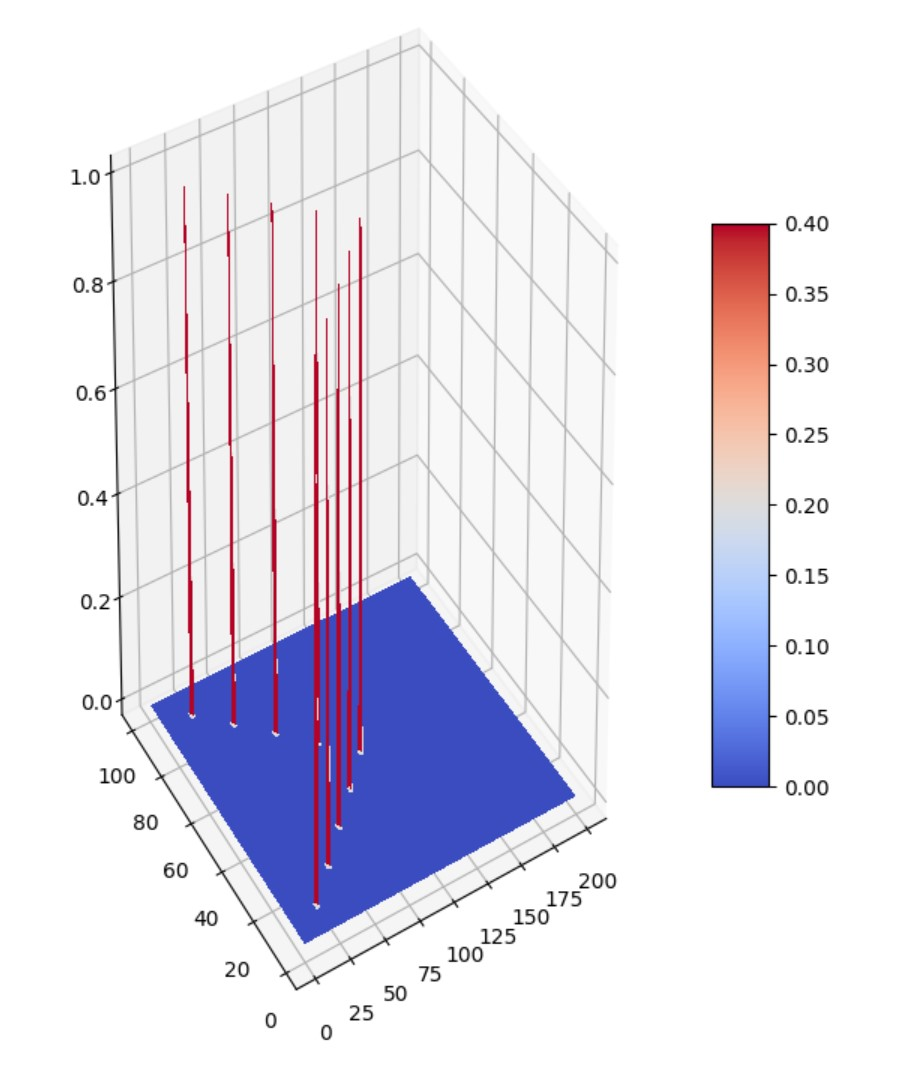
\includegraphics[scale=0.5]{tri1.jpg}
    \caption{The plot of the image as described in question 1c). It forms roughly a triangular shape on the left side of the image}
    \label{fig:my_label}
\end{figure}

\subsection{1 d}

In two dimensions, we define $f(u,v)$ to be some 2-dimensional function that we want to produce as a combination of 2-dimensional impulses. Again we use our defined 2D impulse function $\delta(u,v)$. Using a similar idea to the 1D function sum, we can write:

$$f(u,v) = \sum_{j = 1}^{N} \sum_{i = 1}^{M} f(u_j, v_i)\delta(u - u_j, v - v_i)$$

\noindent
Where we have a $M \times N$ image, and $j$ represents the horizontal coordinate index, while $i$ represents the vertical coordinate index. This is equivalent to scaling each $(i,j)$ position in the image by $f(u_j, v_i)$ (provided that there is an impulse here i.e. this part of the image is not simply black). Thus altogether we get a 2D function $f(u,v)$ represented and scaled by impulses.

\section{Question 2}

\subsection{2 a}

Let $n \times n$ be the image size and $m \times m$ be the convolution filter size. In total there are $n^2$ pixels in the image which the filter will convolve with. The convolution involves $m^2$ operations total, \textit{per pixel}. Therefore, the time complexity of base convolution is $O(n^2 m^2)$.

\subsection{2 b}

Let our initial $m \times m$ filter $h$ be \textbf{separable}. Then we can separate $h$ into a 1D vertical and 1D horizontal filter of size $m$ each, and then only do one pass with each filter. This means instead of $m^2$ operations, we only do $2m$ operations per pixel. This means that our time complexity has been reduced to $O(n^2 2m) = O(m n^2)$.

\subsection{2 c}

We can figure out whether both filters are separable based on singular value decomposition of the matrix. If a matrix's SVD form has only one singular value, then it is separable. We will use the following Python code: 

\begin{lstlisting}
import numpy as np

a = np.matrix('10 40 8; 5 3 5; 12 5 2')
b = np.matrix('6 3 6; 2 1 2; 6 3 6')

U1, s1, V1 = np.linalg.svd(a, full_matrices=True)
U2, s2, V2 = np.linalg.svd(b, full_matrices=True)

print(s1)
print(s2)

\end{lstlisting}

\noindent
From the above code, we see that $F_1$ \textbf{is not separable}, while $F_2$ \textbf{is separable}. The one non-zero singular value is $3 \sqrt{19}$.
\\\\
\noindent
For $F_2$, the horizontal and vertical filters are as follows:

$$F_{2}^{h} = \sqrt{3} \sqrt[4]{19} \begin{bmatrix} 6 & 3 & 6 \end{bmatrix}$$

$$F_{2}^{v} = \sqrt{3} \sqrt[4]{19} \begin{bmatrix} 6 & 2 & 6 \end{bmatrix}^{T}$$

\section{Question 3}

\end{document}